%!TEX root = ../../thesis.tex
\section{Components}

\subsection{Controllers \& Directives}

\begin{figure}[htb]
  \centerline{
    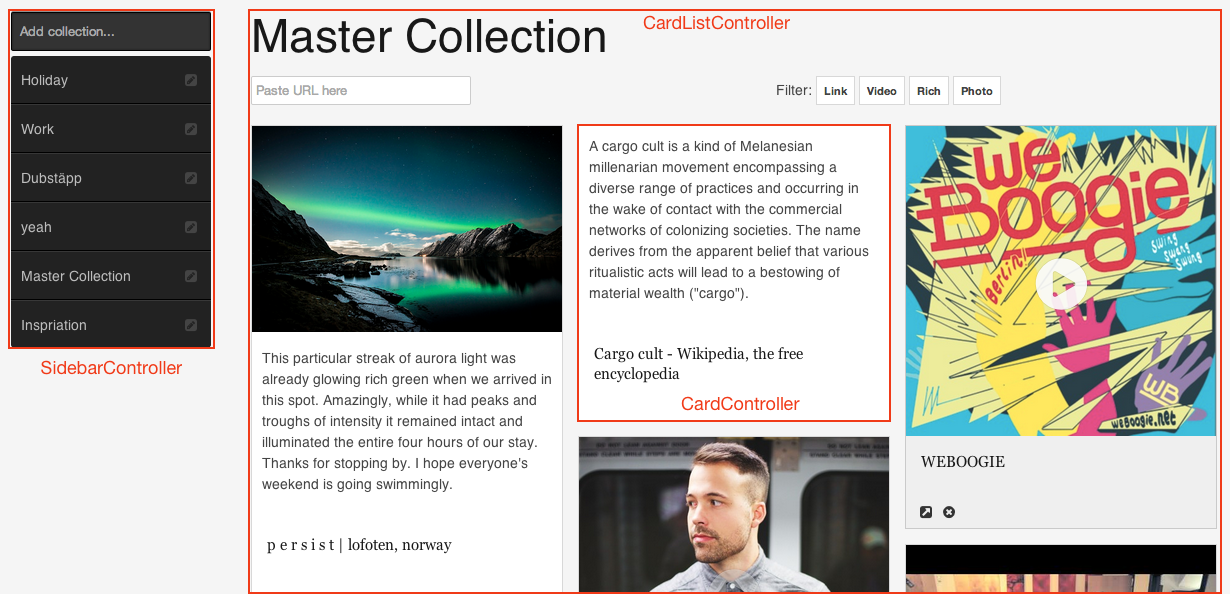
\includegraphics[width=\linewidth]{images/collection-controllers.png}
  }
  \caption[collection.do controllers]{collection.do controllers}
  \label{fig:collection-controllers}
\end{figure}

\begin{figure}[htb]
  \centerline{
    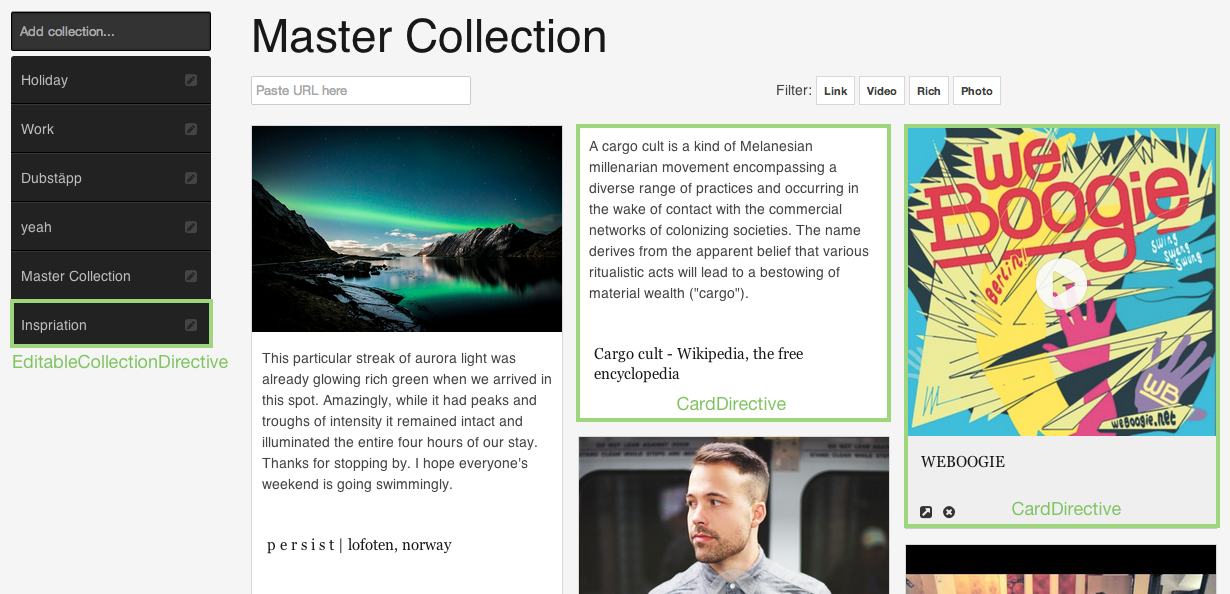
\includegraphics[width=\linewidth]{images/collection-directives.png}
  }
  \caption[collection.do directives]{collection.do directives}
  \label{fig:collection-directives}
\end{figure}

The entire application only consists of four controllers which are all shown in \reffigure{fig:collection-controllers}. For the sidebar there is the \code{SidebarController} which takes care of creating a new collection through the form on the top. It uses the \code{ng-submit} directive to link its method for creating a new collection to the `submit' event of the form: \code{ng-submit=``createNewCollection()''}. In addition to that, it also takes care of loading the content of another collection when they are selected.

Each collection row in the sidebar has its own controller and is based on an own directive as it can be seen in \reffigure{fig:collection-controllers} (EditableController) and in \reffigure{fig:collection-directives} (EditableCollectionDirective). They are used to make collections in this list editable and to delete them. As it has been explained in \refchapter{directive explanation chapter}\todo{write directive chapter}, it makes sense to separate a components DOM methods and its state and logic methods. Following this principle, the \code{EditableCollection} reacts to DOM events in its directive, which trigger the input field's focus method or they end the edit mode (when ESC is being pressed). The methods that actually send the changes to the backend all reside in the controller. Directive and controller communicate by watching the state of an \code{editMode} flag.

The list of cards of a collection is managed by the \code{CardListController} which, depending on the current URL loads the correct collection and its associated items. After the items have been fetched, the \code{ng-repeat} directive in the controller's template renders the individual cards.

\begin{lstlisting}[language=HTML, caption=CardListController template, label=lst:cardlist-template]
  <div ng-repeat="item in filteredItems = 
      (items | filter: cardFilter | orderBy:'-created_at')"
  card></div>
\end{lstlisting}

In this case, the \code{ng-repeat} directive uses a filtered set of elements. It uses the \code{filteredItems} array (line 1, \reflisting{lst:cardlist-template}) which is created by filtering the scope's \code{items} array (line 2). Filters can be applied by using the pipe character and they are executed from left to right. The first filter that is applied to the \code{items} array is the \code{cardFilter} (line 2) which is shown in \reflisting{lst:cardlist-filter}.

\begin{lstlisting}[language=JavaScript, caption=CardListController filter, label=lst:cardlist-filter]
  $scope.cardFilter = function(card){
    if($scope.filter == '') return true;
    return (card.type == $scope.filter);
  };
\end{lstlisting}

A filter function is executed on every item in an array. When the filter function returns \code{false} for an item, it will be removed from the filtered set. It is kept in the set when the filter function returns \code{true}. In the \code{cardFilter} example, the card's \code{type} property is checked if it matches the scope's \code{filter} property (line 3). An empty \code{filter} (line 2) does not remove any card from the set. The \code{filter} property is set by using one of the four buttons on top of the card list (see \reffigure{fig:collection-directives}). After applying the \code{cardFilter}, the built-in \code{orderBy} filter is used to sort the cards by their creation dates (line 2, \reflisting{lst:cardlist-template}).

For each individual card there is again a dedicated controller and a dedicated directive. There are four different kinds of cards in collection.do and all of them are handled in the same template file because all cards basically have the same look, but the content that is displayed in a card varies from type to type. 

\begin{lstlisting}[language=HTML, caption=CardListController template, label=lst:card-template]
<div ng-if="hasImagePreview()" ng-click="showPreview()">
  <span ng-if="hasEmbedContent()">play</span>
  <img ng-src="{{ item.embedlyContent.thumbnail_url }}" />
</div>
\end{lstlisting}

The example shown in \reflisting{lst:card-template} demonstrates the usage of the \code{ng-if} directive that only shows a DOM element if the embedded expression returns \code{true} (line 1). Here, \code{ng-if} is used in combination with controller functions that check if the preview of the card contains certain properties such as an embeddable player (line 2). If an embeddable player is available for the element, the \code{showPreview()} method is used to replace the preview image with an interactive player when the play button is clicked (line 1f). The \code{showPreview} method is part of the directive, because it manipulates the element's DOM content.